\documentclass[a4paper,11pt]{book}
%\documentclass[a4paper,twoside,11pt,titlepage]{book}
\usepackage{listings}
\usepackage[utf8]{inputenc}
\usepackage[spanish]{babel}
\usepackage{float}

% \usepackage[style=list, number=none]{glossary} %
%\usepackage{titlesec}
%\usepackage{pailatino}

\decimalpoint
\usepackage{dcolumn}
\newcolumntype{.}{D{.}{\esperiod}{-1}}
\makeatletter
\addto\shorthandsspanish{\let\esperiod\es@period@code}
\makeatother


%\usepackage[chapter]{algorithm}
\RequirePackage{verbatim}
%\RequirePackage[Glenn]{fncychap}
\usepackage{fancyhdr}
\usepackage{graphicx}
\usepackage{afterpage}
\usepackage{array}
\usepackage{makecell}
\usepackage{tabularray}

\usepackage{longtable}

\usepackage[pdfborder={000}]{hyperref} %referencia

\usepackage[backend=biber, style=numeric, sorting=ynt]{biblatex}


% \usepackage{booktabs}
% \usepackage{dirtree}
% \usepackage{algorithmicx}
% \usepackage{algorithm}
% \usepackage[justification=centering, margin=0.1cm]{caption}
% \usepackage{subcaption}
% \usepackage{multirow}
% \usepackage{enumitem}
% \setlist{nosep}

\newcommand{\INDSTATE}[1][1]{\STATE\hspace{#1\algorithmicindent}}

% \usepackage[
%     a4paper,
%     left=2.8cm,
%     right=2.7cm,
%     top=4cm,
%     bottom=3cm
% ]{geometry}

% ********************************************************************
% Re-usable information
% ********************************************************************
\newcommand{\myTitle}{Detección de errores en bases de datos químicas\xspace}
\newcommand{\myDegree}{Grado en Ingeniería Informática\xspace}
\newcommand{\myName}{Jesús Navarro Merino\xspace}
\newcommand{\myProf}{Rocío Celcete Romero Zaliz\xspace}
%\newcommand{\mySupervisor}{Put name here\xspace}
\newcommand{\myFaculty}{Escuela Técnica Superior de Ingenierías Informática y de
Telecomunicación\xspace}
\newcommand{\myFacultyShort}{E.T.S. de Ingenierías Informática y de
Telecomunicación\xspace}
\newcommand{\myDepartment}{Departamento de ...\xspace}
\newcommand{\myUni}{\protect{Universidad de Granada}\xspace}
\newcommand{\myLocation}{Granada\xspace}
\newcommand{\myTime}{\today\xspace}
\newcommand{\myVersion}{Version 0.1\xspace}


\hypersetup{
pdfauthor = {\myName (email (en) ugr (punto) es)},
pdftitle = {\myTitle},
pdfsubject = {},
pdfkeywords = {palabra_clave1, palabra_clave2, palabra_clave3, ...},
pdfcreator = {LaTeX con el paquete ....},
pdfproducer = {pdflatex}
}

%\hyphenation{}


%\usepackage{doxygen/doxygen}
%\usepackage{pdfpages}
\usepackage{url}
\usepackage{color,colortbl,longtable}
\usepackage[stable]{footmisc}
%\usepackage{index}

%\makeindex
%\usepackage[style=long, cols=2,border=plain,toc=true,number=none]{glossary}
% \makeglossary

% Definición de comandos que me son tiles:
%\renewcommand{\indexname}{Índice alfabético}
%\renewcommand{\glossaryname}{Glosario}

\pagestyle{fancy}
\fancyhf{}
\fancyhead[LO]{\leftmark}
\fancyhead[RE]{\rightmark}
\fancyhead[RO,LE]{\textbf{\thepage}}
\renewcommand{\chaptermark}[1]{\markboth{\textbf{#1}}{}}
\renewcommand{\sectionmark}[1]{\markright{\textbf{\thesection. #1}}}

\setlength{\headheight}{1.5\headheight}

\newcommand{\HRule}{\rule{\linewidth}{0.5mm}}
%Definimos los tipos teorema, ejemplo y definición podremos usar estos tipos
%simplemente poniendo \begin{teorema} \end{teorema} ...
\newtheorem{teorema}{Teorema}[chapter]
\newtheorem{ejemplo}{Ejemplo}[chapter]
\newtheorem{definicion}{Definición}[chapter]

\definecolor{gray97}{gray}{.97}
\definecolor{gray75}{gray}{.75}
\definecolor{gray45}{gray}{.45}
\definecolor{gray30}{gray}{.94}

\lstset{ frame=Ltb,
     framerule=0.5pt,
     aboveskip=0.5cm,
     framextopmargin=3pt,
     framexbottommargin=3pt,
     framexleftmargin=0.1cm,
     framesep=0pt,
     rulesep=.4pt,
     backgroundcolor=\color{gray97},
     rulesepcolor=\color{black},
     %
     stringstyle=\ttfamily,
     showstringspaces = false,
     basicstyle=\scriptsize\ttfamily,
     commentstyle=\color{gray45},
     keywordstyle=\bfseries,
     %
     numbers=left,
     numbersep=6pt,
     numberstyle=\tiny,
     numberfirstline = false,
     breaklines=true,
   }
 
% minimizar fragmentado de listados
\lstnewenvironment{listing}[1][]
   {\lstset{#1}\pagebreak[0]}{\pagebreak[0]}

\lstdefinestyle{CodigoC}
   {
	basicstyle=\scriptsize,
	frame=single,
	language=C,
	numbers=left
   }
\lstdefinestyle{CodigoC++}
   {
	basicstyle=\small,
	frame=single,
	backgroundcolor=\color{gray30},
	language=C++,
	numbers=left
   }

 
\lstdefinestyle{Consola}
   {basicstyle=\scriptsize\bf\ttfamily,
    backgroundcolor=\color{gray30},
    frame=single,
    numbers=none
   }


\newcommand{\bigrule}{\titlerule[0.5mm]}


%Para conseguir que en las páginas en blanco no ponga cabecerass
\makeatletter
\def\clearpage{%
  \ifvmode
    \ifnum \@dbltopnum =\m@ne
      \ifdim \pagetotal <\topskip
        \hbox{}
      \fi
    \fi
  \fi
  \newpage
  \thispagestyle{empty}
  \write\m@ne{}
  \vbox{}
  \penalty -\@Mi
}
\makeatother

\usepackage{pdfpages}


\addbibresource{bibliografia/bibliografia.bib}
% \addbibresource{sample.bib}
% \addbibresource{bibliografia/webs.bib}

\begin{document}
\begin{titlepage}
 
 
\newlength{\centeroffset}
\setlength{\centeroffset}{-0.5\oddsidemargin}
\addtolength{\centeroffset}{0.5\evensidemargin}
\thispagestyle{empty}

\noindent\hspace*{\centeroffset}\begin{minipage}{\textwidth}

\centering

\includegraphics[width=0.9\textwidth]{imagenes/logos/logo_ugr.jpg}\\[1.4cm]

\textsc{ \Large TRABAJO FIN DE GRADO\\[0.2cm]}
\textsc{ INGENIERÍA INFORMÁTICA}\\[1cm]
% Upper part of the page
% 
% Title
\noindent\rule[-1ex]{\textwidth}{2pt}\\[3ex]
{\Huge\bfseries Prueba Detección de errores en bases de datos químicas\\
}
\noindent\rule[-3ex]{\textwidth}{2pt}\\[3ex]
\end{minipage}

\vspace{1.5cm}
\noindent\hspace*{\centeroffset}\begin{minipage}{\textwidth}
\centering

\textbf{Autor}\\ {Jesús Navarro Merino}\\[2.5ex]
\textbf{Directora}\\
{Rocío Celeste Romero Zaliz}\\[2cm]

\includegraphics[width=0.3\textwidth]{imagenes/logos/etsiit_logo.png}\\[0.1cm]
\textsc{Escuela Técnica Superior de Ingenierías Informática y de Telecomunicación}\\
\textsc{---}\\
Granada, julio de 2023
\end{minipage}
%\addtolength{\textwidth}{\centeroffset}
%\vspace{\stretch{2}}
\end{titlepage}


\chapter*{}
%\thispagestyle{empty}
%\cleardoublepage

%\thispagestyle{empty}


% \cleardoublepage
\thispagestyle{empty}

\begin{center}
{\large\bfseries Detección de errores en bases de datos químicas}\\
\end{center}
\begin{center}
Jesús Navarro Merino\\
\end{center}

%\vspace{0.7cm}
\noindent{\textbf{Palabras clave}: Química computacional, Química organometálica, Nomenclatura canónica, SMILES, Representación de moléculas, Cp, OpenBabel, Bases de datos, SciFinder.}\\

\vspace{0.7cm}
\noindent{\textbf{Resumen}}\\

El desarrollo de la informática y la aplicación de sus métodos al mundo de la química ha propiciado grandes avances en esta ciencia. Sin embargo, un campo poco explorado dentro de la química computacional es la organometálica, de manera que muchas de las herramientas existentes no están preparadas para trabajar con ella. En esta área, para los investigadores es importante codificar las moléculas en representaciones lineales como SMILES y usar las herramientas software, para entre otras cosas, representar los compuestos gráficamente y comprenderlos mejor. La heterogeneidad en las distintas bases de datos públicas a la hora de consultar un mismo compuesto entorpece el trabajo de los investigadores.

Tras un análisis de esas inconsistencias, este proyecto propone una nomenclatura canónica para moléculas organometálicas en donde se le dé la suficiente importancia al metal, de manera que quede colocado el primero en el SMILES canónico resultado. En química de coordinación y organometálica, las reacciones y los compuestos no se explican bien siguiendo la teoría del enlace de valencia. Por tanto, se presentan también algunos cambios en el sistema de representación 2D de la herramienta utilizada, para ilustrar de una manera más adecuada los enlaces metal-ligando más habituales en compuestos organometálicos, las estructuras de ciclopentadienilo (Cp). Tras la validación de los resultados con diversos tests de consistencia, se obtienen finalmente resultados satisfactorios.

\cleardoublepage


\thispagestyle{empty}


\begin{center}
{\large\bfseries Error detection in chemical databases}\\
\end{center}
\begin{center}
Jesús Navarro Merino\\
\end{center}

%\vspace{0.7cm}
\noindent{\textbf{Keywords}: Chemoinformatics, Organometallic chemistry, Canonicalization, SMILES, Molecule depiction, Cp, OpenBabel, Databases, SciFinder.}\\

\vspace{0.7cm}
\noindent{\textbf{Abstract}}\\

The development of computer science and the application of its methods to the chemical world has led to great advances in this science. However, a less explored field within computational chemistry is organometallics, meaning that many of the existing tools are not prepared to work with it. In this area, it is important for researchers to encode molecules in linear notations such as SMILES and use software tools to, among other things, depict compounds graphically and have a better understanding of them. Heterogeneity in various public databases when querying the same compound hinders scientists' work.

After an analysis of these inconsistencies, this project proposes a canonical nomenclature for organometallic molecules in which adequate importance is given to the metal, so that it is placed first in the resulting canonical SMILES. In coordination and organometallic chemistry, reactions and compounds do not fit well into the valence bond theory. Therefore, some changes are also presented in the 2D representation system of the tool used, in order to illustrate in a more suitable way the most common metal-ligand bonds in organometallic compounds, cyclopentadienyl (Cp) complexes. After validation of the results with several consistency tests, satisfactory outcomes are finally obtained.

\chapter*{}
\thispagestyle{empty}

\noindent\rule[-1ex]{\textwidth}{2pt}\\[4.5ex]

Yo, \textbf{Jesús Navarro Merino}, alumno de la titulación Grado en Ingeniería Informática de la \textbf{Escuela Técnica Superior
de Ingenierías Informática y de Telecomunicación de la Universidad de Granada}, con DNI 15429457E, autorizo la
ubicación de la siguiente copia de mi Trabajo Fin de Grado en la biblioteca del centro para que pueda ser
consultada por las personas que lo deseen.

\vspace{6cm}

\noindent Fdo: Jesús Navarro Merino

\vspace{2cm}

\begin{flushright}
Granada, a 11 de julio de 2023
\end{flushright}


\chapter*{}
\thispagestyle{empty}

\noindent\rule[-1ex]{\textwidth}{2pt}\\[4.5ex]

Dña. \textbf{Rocío Celeste Romero Zaliz}, Profesora del Departamento de Ciencias de la Computación e Inteligencia Artificial de la Universidad de Granada.


\vspace{0.5cm}

\textbf{Informan:}

\vspace{0.5cm}

Que el presente trabajo, titulado \textit{\textbf{Detección de errores en bases de datos químicas}},
ha sido realizado bajo su supervisión por \textbf{Jesús Navarro Merino}, y autorizamos la defensa de dicho trabajo ante el tribunal que corresponda.

\vspace{0.5cm}

Y para que conste, expiden y firman el presente informe en Granada a 11 de julio de 2023.

\vspace{1cm}

\textbf{La directora:}

\vspace{5cm}

\noindent \textbf{Rocío Celeste Romero Zaliz}

\chapter*{Agradecimientos}
\thispagestyle{empty}

       \vspace{1cm}


A mi tutora Rocío, por su esfuerzo y guía a lo largo del proyecto. Por su paciencia y ánimos en los momentos más críticos.
\\

A mis amigos, que por los buenos momentos vividos y el día a día con ellos, han hecho que estos años en la universidad hayan pasado casi sin darme cuenta.
\\

Y a mis padres, por su apoyo incondicional y confianza durante todo este trayecto. 
\frontmatter
\tableofcontents
\listoffigures
\renewcommand{\listtablename}{Índice de tablas}
\renewcommand{\tablename}{Tabla}
\listoftables

\mainmatter
\setlength{\parskip}{5pt}

\chapter{Introducción}




% \begin{tblr}{|Q[h,t]|Q[c,t]|Q[r,b]|}
% \hline
% {C[Au].c1ccc(cc1)P(c2ccccc2)c3ccccc3 \\ Left Left} & Middle Center & {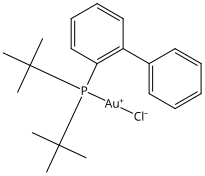
\includegraphics{imagenes/SciFinder/Chloro[(1,1-biphenyl-2-yl)di-tert-butylphosphine]gold(I).png}} \\
% \hline
% \end{tblr}

\textbf{Meter aqui una introduccion general sobre la química, la quimica informatica (y cómo surge en base a las necesidades computacionales), mencionar brevemente la organometalica (mas tarde en la seccion de estado del arte profundizo, junto con cosas de dibujado, tutorial de SMILES, y representacion de moléculas)}


\section{Motivación y objetivos}

Los formatos de notación lineal llevan siendo un tema de interés e investigación para los científicos desde mediados del siglo 19 \cite{107_years_linear_notations} \textbf{Terminar esto}

En la actualidad, existen varias representaciones lineales \textbf{(Para esto debo haber hablado antes de las representaciones lineales, o bien lo explico aquí, o bien lo redirijo a los fundamentos teóricos. O bien, justo antes de empezar este párrafo, que será lo mejor-> quitar entonces la siguiente negrita)}, siendo las más usadas SMILES, InChI, y SELFIES \cite{SELFIES}. \textbf{Como comenté antes, una forma muy potente de representar moléculas y compuestos químicos es mediante cadenas strings}, y de esto justamente se encargan las representaciones lineales: traducir una molécula, con sus átomos, enlaces entre ellos, ciclos y otras propiedades características, en una cadena string que la represente, y que la máquina y los propios químicos puedan entender. Sin embargo, hay diferencias notables entre las representaciones, tanto en la sintaxis de las cadenas que se generan como en las aplicaciones que se le puede dar a cada una de ellas.

SMILES, ideada por David Weininger, sale a la luz en 1988 satisfaciendo con creces las necesidades de procesamiento de información química que había, desbancando a la representación estandarizada del momento, Wiswesser Line Notation (WLN). Desde ese entonces SMILES se convirtió —y sigue siendo a día de hoy— en el estándar de representación lineal, ya que permite describir estructuras moleculares de una forma sencilla en un formato fácil de leer, lo que ha hecho que sea una herramienta popular en la química computacional, siendo la más usada entre investigadores y químicos. Pese a esto, SMILES tiene dos grandes inconvenientes: una misma molécula puede escribirse con varias cadenas SMILES distintas válidas, es decir, tiene sinónimos (Figura \ref{fig:sinonimos_smiles}); y no es robusto ni sintáctica ni semánticamente. En este sentido se podría generar un string que no represente una molécula válida, como lo es \emph{CC(CCCC}, el cual tiene un paréntesis sin cerrar (lo que implica que no se delimita cuándo acaba la rama). O generar una molécula que no sea químicamente viable como \emph{CO=CC}, que muestra un átomo de oxígeno neutro formando tres enlaces (superando el límite de enlaces covalentes que un oxígeno neutro puede tener) \cite{SELFIES}.

\begin{figure}[H]
\centering
    \fbox{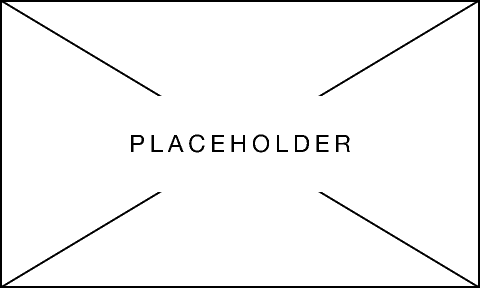
\includegraphics[scale=0.3]{imagenes/placeholder.png}}  
    \caption{Distintas cadenas SMILES válidas para la misma molécula de <nombre-molecula>. \cite{}}
    \label{fig:sinonimos_smiles}
\end{figure}

Esto tiene especial relevancia en el ámbito del Machine Learning (ML). Aunque se sale del alcance de este trabajo, uno de los grandes objetivos de la química computacional es la creación o diseño de nuevas moléculas. Se podrían crear modelos de ML o redes neuronales capaces de generar moléculas ficticias válidas, para posteriormente ver sus propiedades, valorarlas energéticamente para ver cuán estables son, y estudiar su viabilidad en distintas aplicaciones, entre otras cosas. SMILES dificulta esta tarea, y por ello, aparece en 2020, SELFIES (SELF-referencIng Embedded Strings), una nueva representación lineal 100\% robusta, muy usada actualmente para modelos generativos. Ver \cite{SELFIES, krenn_self_referencing_2020} para más detalles de cómo soluciona los problemas de robustez y otras características de la representación. SELFIES es relativamente reciente y continuamente está ampliando sus funcionalidades, mejorando su simplicidad y facilidad de uso para el usuario \cite{selfies_recent_2023}. Aun así, no se termina de instaurar entre la comunidad investigadora. 

\textbf{AQUI METER ALGO DE InChI, o lo meto arriba, antes de hablar sobre SELFIES.
}

Por todo lo anterior, me centraré en la notación SMILES durante el desarrollo de este trabajo. Dicho esto, existen diversas fuentes de datos en química donde se recoge gran cantidad de información acerca de los compuestos. Menciono las más importantes y las que serán objeto de interés. \emph{PubChem}, una base de datos abierta que sirve información a millones de usuarios en todo el mundo, desde investigadores y estudiantes hasta el público general. Recogen para cada compuesto, información sobre su estructura, representaciones 2D y 3D, identificadores, propiedades químicas y físicas, patentes, avisos de toxicidad, etc. \cite{pubchem_website} 

\emph{SciFinder}, una herramienta de investigación muy potente que permite explorar las bases de datos de CAS (American Chemical Society) las cuales contienen literatura sobre Química y otras disciplinas afines como Física, Biomedicina, Geología, Ingeniería Química, etc. Incluye referencias bibliográficas y resúmenes de artículos, informes, y libros entre otras cosas. Permite realizar búsquedas por estructura, nombres de sustancias o identificadores, reacciones en la que participa dicha sustancia, artículos y publicaciones que nombren el compuesto en cuestión, e incluso proveedores de compra. Para el uso de esta herramienta es necesario acceder mediante la red de una institución autorizada (en este caso trabajo mediante VPN de la UGR) y seguir los pasos para registrarte \footnote{Pasos para el registro en SciFinder \url{https://bibliotecaugr.libguides.com/scifinder_scholar}}

uno de los principales problemas que se detectan es la heterogeneidad en las distintas bases de datos \textbf{continuar esto}



\textbf{Aquí empezar ya con la tabla comparativa. Para eso, tengo que introducir las fuentes de datos }

\noindent \textbf{Meter parrafo de los quimicos colaboradores...mirar pedro}

Por todo lo anterior, una solución que permita aunar... \textbf{continuar esto}  

Por tanto, el objetivo principal de este Trabajo Fin de Grado sería modificar el paquete OpenBabel creando un método para canonizar códigos SMILES, orientado específicamente para compuestos organometálicos, de los cuales dispongo de un conjunto de datos de 30 moléculas considerados de interés por la tutora y los químicos con los que colabora. Para ello, se establecen los siguientes subobjetivos:
\begin{itemize}
    \item Analizar y comparar las cadenas SMILES de distintas bases de datos (p.ej. Sigma-Aldrich, SciFinder) viendo los posibles sinónimos para una misma molécula.
    \item Determinar un sistema que genere, a partir de cualquier sinónimo SMILES de la misma molécula, un único SMILES canónico.
    \item Definir otro algoritmo o conjunto de reglas que mejore, aunque sea mínimamente, el sistema de dibujado de los compuestos.
\end{itemize} 



\begin{table}
\small
  \begin{tabular}
      {lc} \hline Código SMILES & Representación 2D \\ \hline C[Au].c1ccc(cc1)P(c2ccccc2)c3ccccc3 & \parbox[c]{5em}{
      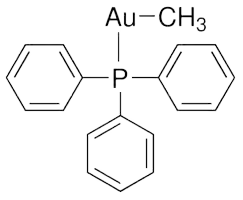
\includegraphics[width=2cm]{imagenes/SigmaAldrich/Methyl(triphenylphosphine)gold(I).png}} \\ \hline
      Cl[Pd]Cl.C1CC=CCCC=C1 & \parbox[r]{5em}{
      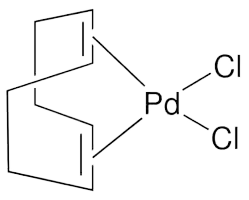
\includegraphics[width=2cm]{imagenes/SigmaAldrich/Dichloro(1,5-cyclooctadiene)palladium(II).png}} \\ \hline
      Cl[Au].CP(C)C & \parbox[c]{5em}{
      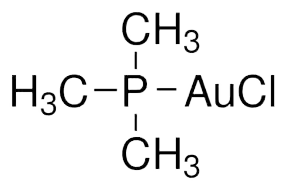
\includegraphics[width=2cm]{imagenes/SigmaAldrich/Chloro(trimethylphosphine)gold(I).png}} \\ \hline
      Cl[Au].CC(C)(C)P(c1ccccc1-c2ccccc2)C(C)(C)C & \parbox[c]{5em}{
      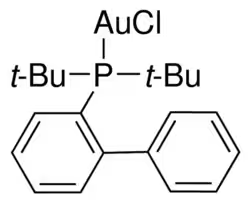
\includegraphics[width=2cm]{imagenes/SigmaAldrich/Chloro[(1,1-biphenyl-2-yl)di-tert-butylphosphine]gold(I).png}} \\ \hline
      [Fe]I.[C-]\#[O+].[C-]\#[O+].[CH]1[CH][CH][CH][CH]1 & \parbox[c]{5em}{
      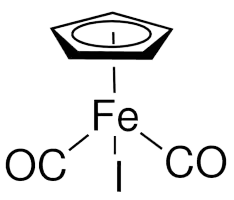
\includegraphics[width=2cm]{imagenes/SigmaAldrich/Dicarbonylcyclopentadienyliodoiron(II).png}} \\ \hline
  \end{tabular}
  \caption{Códigos SMILES y sus representaciones 2D según Sigma-Aldrich}
\end{table}


\begin{table}
\small
  \begin{tabular}
      {lc} \hline Código SMILES & Representación 2D \\ \hline 
      [Au+]([CH3-])[P](C=1C=CC=CC1)(C=2C=CC=CC2)C=3C=CC=CC3 & \parbox[c]{5em}{
      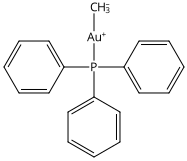
\includegraphics[width=2cm]{imagenes/SciFinder/Methyl(triphenylphosphine)gold(I).png}} \\ \hline
      [Cl-][Pd+2]123([Cl-])[CH]=4CC[CH]3=[CH]2CC[CH]41 & \parbox[r]{5em}{
      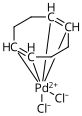
\includegraphics[width=2cm]{imagenes/SciFinder/Dichloro(1,5-cyclooctadiene)palladium(II).png}} \\ \hline
      [Cl-][Au+][P](C)(C)C & \parbox[c]{5em}{
      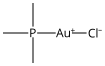
\includegraphics[width=2cm]{imagenes/SciFinder/Chloro(trimethylphosphine)gold(I).png}} \\ \hline
      [Cl-][Au+][P](C=1C=CC=CC1C=2C=CC=CC2)(C(C)(C)C)C(C)(C)C & \parbox[c]{5em}{
      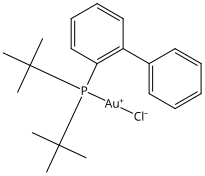
\includegraphics[width=2cm]{imagenes/SciFinder/Chloro[(1,1-biphenyl-2-yl)di-tert-butylphosphine]gold(I).png}} \\ \hline
      O\#C[Fe+2]1234([I-])(C\#O)[CH]=5[CH]4=[CH]3[CH-]2[CH]51 & \parbox[c]{5em}{
      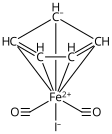
\includegraphics[width=2cm]{imagenes/SciFinder/Dicarbonylcyclopentadienyliodoiron(II).png}} \\ \hline
  \end{tabular}
  \caption{Códigos SMILES y sus representaciones 2D según SciFinder}
\end{table}








\begin{table}
  \begin{tblr}
      {Q[c,t]Q[c,m]} \hline Código SMILES & Representación 2D \\ \hline 
      C[Au].c1ccc(cc1)P(c2ccccc2)c3ccccc3 & 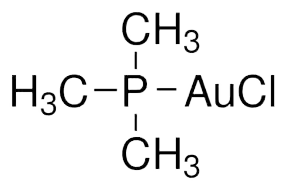
\includegraphics[width=2cm]{imagenes/SigmaAldrich/Chloro(trimethylphosphine)gold(I).png}
       \\
      Cl[Pd]Cl.C1CC=CCCC=C1 & 
      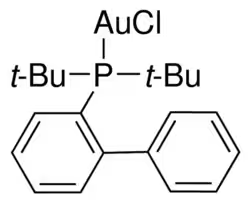
\includegraphics[width=2cm]{imagenes/SigmaAldrich/Chloro[(1,1-biphenyl-2-yl)di-tert-butylphosphine]gold(I).png} \\
      Cl[Au].CP(C)C & 
      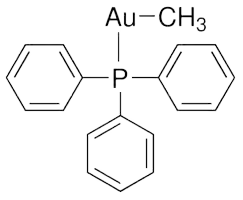
\includegraphics[width=2cm]{imagenes/SigmaAldrich/Methyl(triphenylphosphine)gold(I).png} \\
      Cl[Au].CC(C)(C)P(c1ccccc1-c2ccccc2)C(C)(C)C & 
      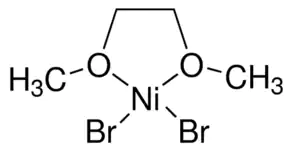
\includegraphics[width=2cm]{imagenes/SigmaAldrich/Nickel(II) bromide ethylene glycol dimethyl ether complex.png} \\ [0cm]
    [Fe]I.[C-]\#[O+].[C-]\#[O+].[CH]1[CH][CH][CH][CH]1 & 
      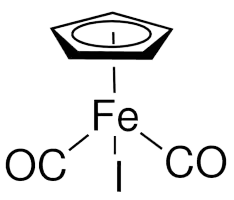
\includegraphics[width=2cm]{imagenes/SigmaAldrich/Dicarbonylcyclopentadienyliodoiron(II).png} \\ \hline
  \end{tblr}
  \caption{Códigos SMILES y sus representaciones 2D según Sigma-Aldrich}
\end{table}


% \begin{longtblr}{
%   colspec={Q[valign=t]Q[valign=b]Q[valign=h]},
%   row{1}={halign=c},
%   hlines
% }
% Id & Name & Figure \\
% 1 & Press imaginary a button & 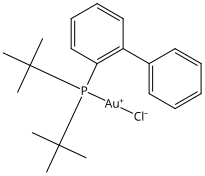
\includegraphics{imagenes/SciFinder/Chloro[(1,1-biphenyl-2-yl)di-tert-butylphosphine]gold(I).png}\\ 
% 1 & Press imaginary a button & 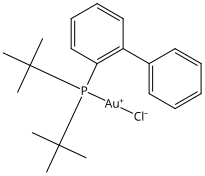
\includegraphics{imagenes/SciFinder/Chloro[(1,1-biphenyl-2-yl)di-tert-butylphosphine]gold(I).png}\\
% 1 & Press imaginary a button & 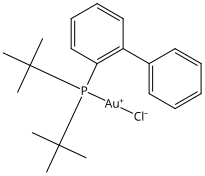
\includegraphics{imagenes/SciFinder/Chloro[(1,1-biphenyl-2-yl)di-tert-butylphosphine]gold(I).png}\\
% 1 & Press imaginary a button & 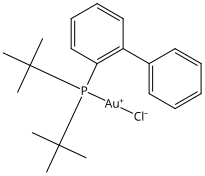
\includegraphics{imagenes/SciFinder/Chloro[(1,1-biphenyl-2-yl)di-tert-butylphosphine]gold(I).png}\\
% 1 & Press imaginary a button & 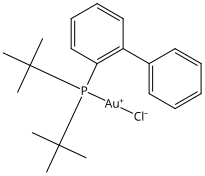
\includegraphics{imagenes/SciFinder/Chloro[(1,1-biphenyl-2-yl)di-tert-butylphosphine]gold(I).png}\\
% 1 & Press imaginary a button & 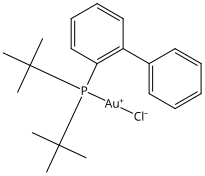
\includegraphics{imagenes/SciFinder/Chloro[(1,1-biphenyl-2-yl)di-tert-butylphosphine]gold(I).png}\\
% \end{longtblr}

\section{Objetivos}


\section{Estructura de la memoria}

% \begin{table}[ht]
%     \centering
%     \begin{tabular}{p{0.35\linewidth} | p{0.6\linewidth}}
%       Column 1  & Column2 \\ \hline
%       This text will be wrapped & Some more text \\
%       Some text here & This text maybe wrapped here if its tooooo long \\
%     \end{tabular}
%     \caption{Caption}
%     \label{tab:my_label}
% \end{table}


\chapter{Estado del arte y fundamentos teóricos}

Quizas sea mejor mover esta seccion justo despues de la introduccion para seguir con la tematica de la motivacion, y ya luego me meto con la gestion y planificacion

Puedo hacer una revision de la literatura existente hasta dia de hoy sobre el tema
Usar SCOPUS para esto, con terminos tipo: "SMILES" "molecule" "organometalic" (juntarlos o separarlos segun vea)

Hablar por aqui de la organometalica, representacion de moléculas, Hablar mas extendido de SMILES, SELFIES, e INCHI; cosas de dibujado de moleculas (los paquetes que hay), )
No se si meterlo aqui o en otro apartado, el diagrama de clases

la historia de la humanidad está marcada por la búsqueda de materiales que mejoren su calidad de vida, y los metales han sido parte crucial de esos cambios 

La materia que forma los seres vivos tiene en su composición sustancias cuya base I principal es el carbono. El estudio de estos compuestos constituye una rama de la química llamada química orgánica. La abundancia del carbono en el planeta es relativamente pequeña: aproximadamente un 0,03 \%; sin embargo, da lugar a millones de sustancias diferentes, mientras que los compuestos inorgánicos son solo unos pocos miles. ¿Qué hace a este elemento tan especial? Su estructura singular, que le permite formar largas cadenas en las cuales una pequeña variación da lugar a un compuesto distinto al anterior.


(del archivo de informeReuniones puedo ir sacando cosas para meter en el estado del arte) Openbabel como tal no soporta el dibujado en 3D de las moléculas, por lo que los únicos dibujos que puede hacer son en 2D. Openbabel tampoco soporta el uso de wedge ni hash bonds para el dibujado de moléculas en 2D con perspectiva (es curioso porque en el código sí que hay funciones dedicadas a esto, pero luego cuando le metes símbolos SMILES de @@ y demás, los medio ignora. Sigo ejemplos del tutorial de Daylight, pero no salen los mismos dibujos. Otros símbolos más dedicados a geometría que viene en Daylight o en OpenSMILES, tipo @SP, @TB, @OH, los ignora por completo). Pero sí es capaz de generar archivos .sdf con información 3D, que se pueden usar en otros softwares de dibujado específicos como Avogadro (y no están mal, mucho mejor que los 2D desde luego)

\bigskip

\chapter{Gestión y Planificación del proyecto}



\section{Metodología}


\section{Gestión de recursos}

\subsection{Recursos humanos}

\subsection{Recursos materiales}

\subsection{Recursos software}

\section{Gestión de costes}

\subsection{Coste de recursos humanos}
Esto quizás dejarlo para el final, cuando tenga la cantidad total de horas trabajadas (aunque podría hacerlo con las "300"horas que se supone que le tengo que dedicar)


\subsection{Coste hardware}

\subsection{Otros costes}

\subsection{Presupuesto final}


\section{Análisis de riesgos}






% \input{capitulos/Diseno_e_implementacion.tex}

\chapter{Experimentación}

Aquí la idea es ir poniendo las pruebas que vaya haciendo de las moléculas, y lo que vaya descubriendo. Problablemente exponer aqui tb el método o reglas de canonizacion a las que llegue.

\input{capitulos/Conclusiones.tex}


% El nocite* es para que muestre todos los elementos de la bibliografia, aunque no se hayan usado para citar nada en el documento (usando \cite{})
% \nocite{*}
\printbibliography[title={Bibliografía}]
% \printbibliography{sample.bib}
% \printbibliography[type=online, title={Otras fuentes}]

% \printbibheading
% \printbibliography{nottype=misc, heading=subbibliography, title={Citas}}
% \printbibliography{type=misc, heading=subbibliography, title={Otras fuentes}}


% \nocite{*}
% \bibliography{sample}
% \bibliographystyle{ieeetr}
% \addcontentsline{toc}{chapter}{Bibliografía}
% \bibliographystyle{miunsrturl}
%
%\appendix
%\input{apendices/manual_usuario/manual_usuario}
%%\input{apendices/paper/paper}
%\input{glosario/entradas_glosario}
% \addcontentsline{toc}{chapter}{Glosario}
% \printglossary
% \chapter*{}
\thispagestyle{empty}

\end{document}